%!TEX program = xelatex
\documentclass[12pt]{article}
\usepackage{amsmath}
\usepackage[usenames,dvipsnames,svgnames,table]{xcolor}
\usepackage[colorlinks=true,urlcolor=blue,linkcolor=blue]{hyperref}
\usepackage{graphicx}
\usepackage{titlesec}
\usepackage[raggedright]{sidecap}
\sidecaptionvpos{figure}{c}
\usepackage{ifxetex}
\ifxetex
\usepackage{mathspec}
\usepackage{xunicode}
\defaultfontfeatures{Mapping=tex-text}
\defaultfontfeatures{Ligatures=TeX}
% \setromanfont{Iowan Old Style Roman}
\setsansfont{PT Sans}
% \setmathfont{XITS Math}
% \setmathrm{XITS Math}
\setmonofont[Scale=0.8]{Menlo}
\else
\usepackage[utf8]{inputenc}
\usepackage[T1]{fontenc}
\fi

% Section header formatting
\titleformat{\section}
  {\normalfont\sffamily\Large\bfseries\color{DarkSlateBlue}}
  {\thesection}{1em}{}
\titleformat{\subsection}
  {\normalfont\sffamily\large\bfseries\color{SteelBlue}}
  {\thesubsection}{1em}{}

% Commands, aliases, etc
\graphicspath{{./figs/}{./}}
\DeclareMathOperator*{\argmin}{argmin}

\title{\sffamily\bfseries{Software alignment of PHENIX VTX detector using the Millepede II package}}
\author{\sffamily{Andrew Adare, Darren McGlinchey, Jin Huang, Jamie Nagle}}
% \author{\fontspec{Helvetica Neue}{Andrew Adare, Darren McGlinchey, Jin Huang}}
\date{\sffamily{\today}}
\begin{document}
\maketitle
\section{Introduction}
The PHENIX VTX detector is designed to locate primary and secondary vertices with a precision of xxx um as well as significantly improve tracking performance in conjunction with other detectors. A software model of the VTX sensors is required during track reconstruction from raw hits. This geometry modeled in the software must reflect the actual position of the VTX sensor planes to within a few tens of microns in order to achieve design resolution in quantities such as the distance of closest approach (DCA) between tracks and the primary vertex. Direct measurements of the sensor planes through surveys can help, but the most precise method for obtaining the correct detector geometry is to use the reconstructed tracks themselves---or more precisely, the distance between track projections and measured hits on a sensor plane. These distances are referred to as ``pulls'' or residuals.

A traditional method of aligning the detector is to histogram the residuals, then directly adjust the position of the detector units such that the residual distributions are centered at zero, with the smallest variance possible. This method handles each detector unit independently, and as such, there is no explicit notion of a global optimum. If one sensor is only partially functional, it is still relocated with equal weight as a fully operational sensor, despite its potentially larger uncertainty or bias. 

In addition, the sensitive direction the sensors is highly anisotropic in space. For example, the VTX sensors are sensitive primarily in the azimuthal and longitudinal directions. This means that there are strong constraints on certain coordinates and weak constraints in others, depending on sensor and track positions and orientations. The traditional method does not provide a way to properly take this into account.

In PHENIX, the traditional method uses SvxCentralTracks, which are projected inward from the Drift Chamber and used as a seed for VTX cluster association. This external information TODO finish this sentence

The Millepede package was designed to alleviate these problems by minimizing a global objective rather than handling the detector sub-units in isolation. It works by collecting a large number of residuals, each associated with their own ``local fit object'' (i.e. a track), then trying out various combinations of global parameters (i.e. sensor positions) to find the configuration that minimizes the total overall (squared) distance between the track projections and measured hits. Like many optimization packages, there are a few qualifications: (a) Millepede can only provide a local minimum, and (b) a correct gradient of the objective with respect to each parameter must be provided by the user. In complicated geometries, the latter point can be one of the more difficult parts about getting Millepede to work right.

This document describes how Millepede was used to self-align the VTX in Run 14, hopefully in sufficient detail that the next person can get through it without too much trouble.

\begin{figure}[tb]
  \begin{center}
    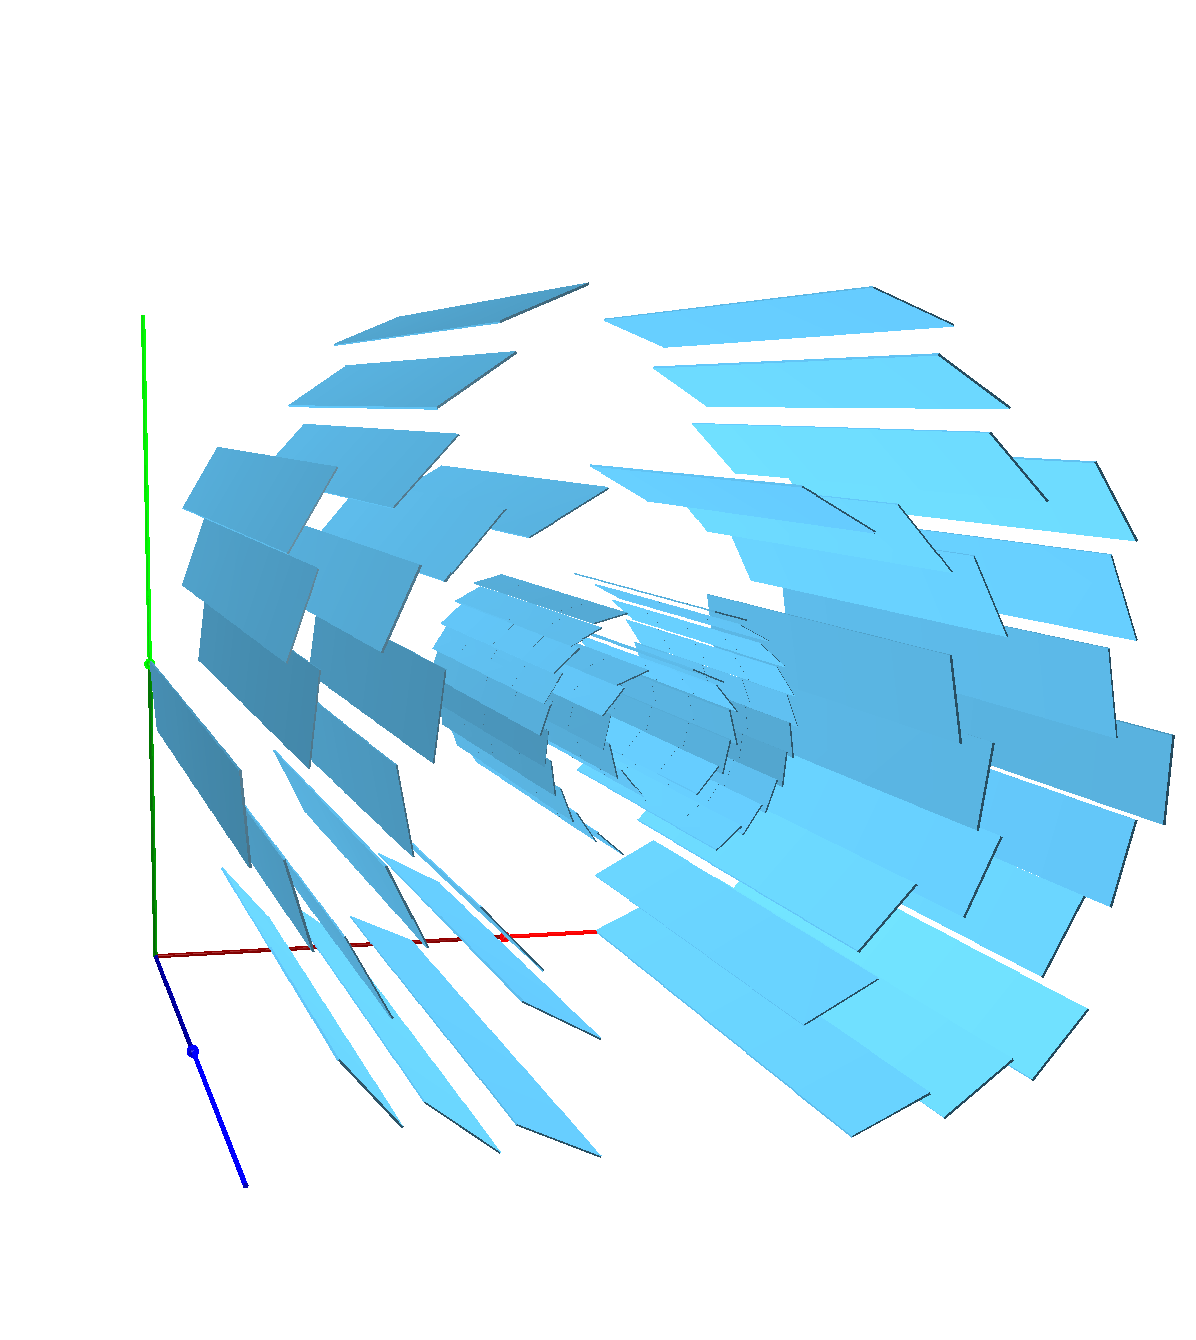
\includegraphics[width=0.45\textwidth]{viewer}
    \quad
    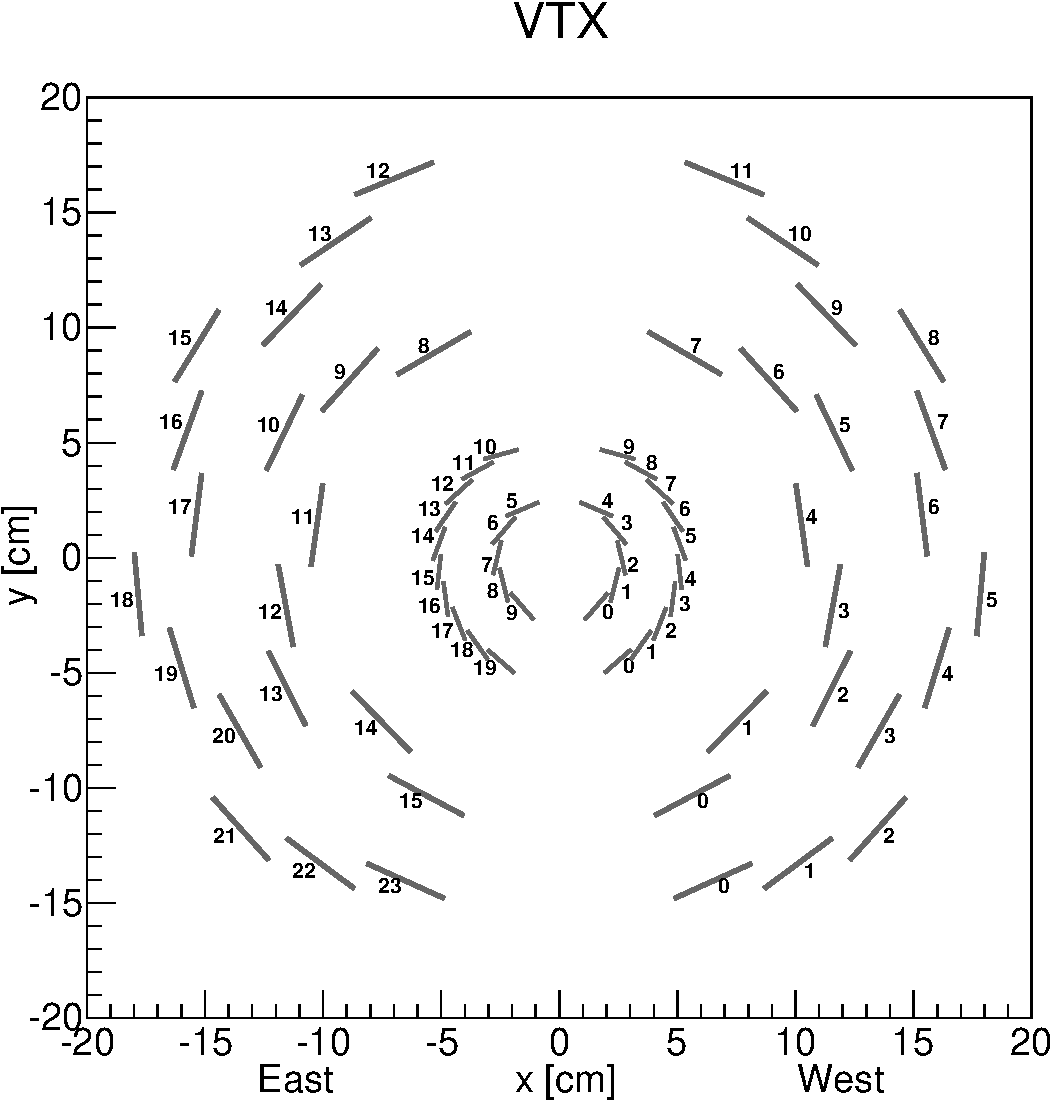
\includegraphics[width=0.5\textwidth]{vtx-xy}
  \end{center}
  \caption{Left: image from 3D viewer in \texttt{svxgeo/examples/DrawVtx.C}. Right: end-on view with ladder and arm labeling scheme.}
  \label{fig:vtx}
\end{figure}

\section{VTX geometry and alignment parameters}
The VTX has a roughly concentric cylindrical geometry, as shown in figure~\ref{fig:vtx}. It consists of 4 barrel layers numbered 0-3, and divided into east and west halves or ``arms''. There are $10+20+16+24 = 70$ ladders in layers 0-3. The ladders are divided equally between the two arms, so that e.g. W0 is a halflayer that contains ladders 0-4; E0, 5-9. For our purposes, a ladder is the finest individual geometric unit.

The ladders are configured such that they overlap slightly as encountered on a radial path outward from the beamline. This is an important feature for self-alignment of the VTX, because the overlaps lead to topological connections between different azimuthal regions. Without coupling between ladders in the azimuthal direction, ladder-by-ladder self-alignment would be very difficult or impossible. 
\vspace{-2cm}
\begin{SCfigure}[50][htb]
\centering
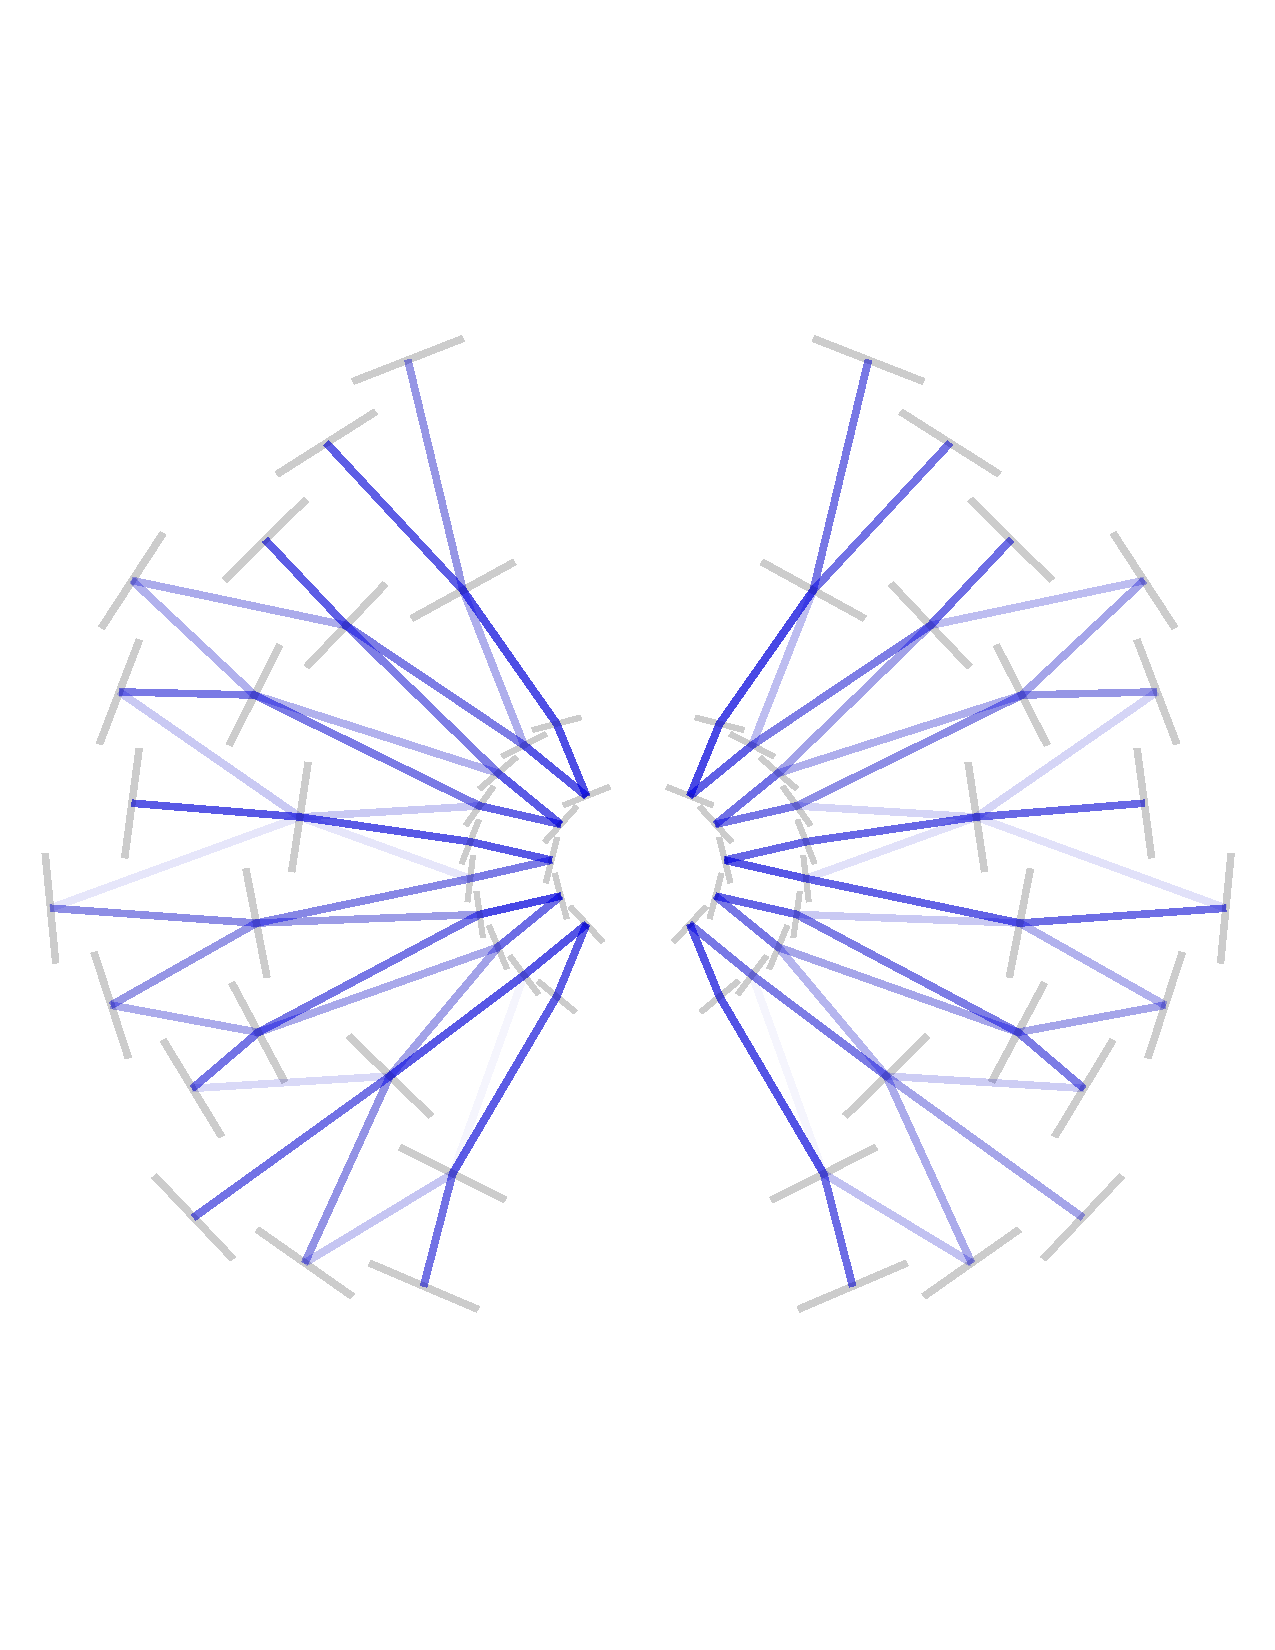
\includegraphics[width=0.6\textwidth]{topology}
\caption{Topology of connected ladders from $10^4$ simulated tracks. The lines are created between ladders that are connected by a straight-line track originating from $(v_x, v_y) = (0,0)$, and the transparency of the lines represents the number of tracks making the connection.}
\label{fig:topo}
\end{SCfigure}
\vspace{-2cm}
A diagram of this connectivity is shown in figure~\ref{fig:topo}, where a distinct web-like connection pattern is clearly visible. Without overlaps, a spoke-like pattern would be visible instead.

\subsection{\texttt{libsvxgeo}} \label{sec:svxgeo}
Fortunately, the VTX geometry can be composed from nothing more than a bunch of rectangular volumes. The geometry model and manipulations are handled by the SvxTGeo class, which in turn leverages the geometry tools included by default with ROOT. This package resides in CVS at \href{https://www.phenix.bnl.gov/viewvc/viewvc.cgi/phenix/offline/packages/svxgeo}{\texttt{offline/\-packages/\-svxgeo}}.

As with other detector geometry software packages like GEANT, the geometry is conceptually modeled using a tree data structure, with the top node representing a reference frame like the experiment hall. Detector elements are grouped or nested within larger units, and their positions and orientations need only be specified with respect to their parent node. Position of any element in the global reference frame can thus be computed at any time by a composition of translations and rotations up the node tree. This is all handled by library functions in ROOT's geometry classes.

The node tree in SvxTGeo is particularly shallow: under the top volume, there are only sensors. This is also more or less the case in the VTX PISA framework.
There are no explicit ladder nodes or volumes. Instead, the sensors are locked together to effectively create ladders when needed. Thus, all manipulations currently available in the SvxTGeo class move only ladders, halflayers, or arms.

In addition to SvxTGeo, there is an SvxProj class that can be used to simulate track hits in the VTX geometry, given a track with an initial angle (and momentum, if $B \neq 0$). In particular, \texttt{SvxProj::FindHitsFromVertex()} can be used to compute residuals from simulated in a geometry with known misalignment. This was used extensively to understand and debug the Millepede alignment process, and is recommended for gaining insights in future alignment projects.

\section{Millepede II}
The \href{http://www.desy.de/~kleinwrt/MP2/doc/html/index.html}{Millepede II} package version 04-01-01 was used for Run 14. It was compiled using GCC 4.6 on Mac OS X 10.9. (Note that Clang/LLVM does not natively support Fortran compilation at this time.)

Millepede II consists of two components, \texttt{mille} and \texttt{pede}. The first is responsible for collecting alignment data and writing it to a binary file for input to \texttt{pede}. It is available as a C++ class, and is packaged with the \texttt{vtx-align} software for convenience (see section~\ref{sec:vtxalign}). The second is a static executable accepting a configuration file name as a command-line argument.

\section{VTX alignment software} \label{sec:vtxalign}
The \texttt{vtx-align} package is kept on the \href{https://git.racf.bnl.gov/phenix/cgit/vtx-align/vtx-align.git}{RCF Git repository}. There is some C++11 code scattered throughout, so ROOT 6 is required. 

The only dependency is \texttt{libsvxgeo} (see section~\ref{sec:svxgeo}) and a file called \texttt{UtilFns.h} used for plotting, i/o, and other generic tasks. This file is available at \href{https://github.com/andrewadare/utils.git}{the author's github site}. (TODO: I should probably just add this into vtx-align)

\subsection{Software layout}
The code was deliberately designed to be as simple and flexible as possible: all reusable code is encapsulated in functions residing in various header files without namespace qualification. Outside of function signatures, there are very few global variables. During execution, the majority of the mutable program state is held in a single object (\texttt{geoEvents}), which is simply a nested STL vector of \texttt{SvxGeoTrack} objects. VtxIO.h contains the code to go from a geoEvents object to TTree storage or vice versa.

For a small software project, this is by far simpler and more flexible than encapsulating data in a heirarchical object-oriented framework. There are a few downsides: it may be inobvious at times where some functions are defined, and the global namespace may get crowded if many headers are included. But these were not problems in practice, and this model worked extremely well for this project.

\subsection{\texttt{VtxAlign.C}}
The core script interfacing with \texttt{Mille} and \texttt{pede} is \texttt{VtxAlign.C}. In a nutshell, it does the following:
\begin{enumerate}
  \item Read in the VTX geometry from a text file and create an SvxTGeo model
  \item Specify the detector sub-units to be aligned (arm, halflayer, ladder) and their allowed degrees of freedom. Together, this is the list of global parameters.
  \item Read in track/residual data as a \texttt{geoEvents} object
  \item Write a text file listing the global parameter constraints
  \item Write a steering file for input to \texttt{pede}
  \item Run \texttt{Mille::mille()} to generate a binary input file
  \item Run \texttt{pede}
  \item Apply the recommended geometry corrections
  \item Refit the tracks in the new geometry, update the residuals, and store the results.
\end{enumerate}
This script is designed to be run iteratively, and the results are stored and plotted at each step to track progress.

\section{Fitting tracks in zero-field data} \label{sec:trackfit}
For self-alignment of the VTX, the PHENIX standalone tracking software is used for association of hits to common track stubs, and little else. Given a set of hits that have already been associated to a track in zero-field data, the task of finding the track parameters by fitting to 3 or 4 hits (plus a vertex or beamcenter position) is simple and fast to compute.

\subsection{Decomposition of fit into two planes} \label{sec:fitdecomp}
Each track is fit separately in the azimuthal plane and in the radial-longitudinal plane. This involves constructing two simple linear functions. First, the azimuthal equation is
\begin{equation} \label{eq:yxfit}
y'(x') = y_0' + m' x'.
\end{equation}
In equation~\ref{eq:yxfit}, the primes indicate rotation of the track within the detector coordinate system. They are introduced for the following reason: ordinary least squares fitting requires that the errors be parallel to the dependent coordinate axis, but in the $x$-$y$ plane, the resolution lies along the azimuthal direction (which, of course, is only aligned with $y$ at $\phi \approx 0$). To rectify this, the track is simply rotated ``backwards'' about the $z$ axis by its approximate azimuthal angle $\phi_{rot}$ such that it points along the $x$ axis. To be explicit,
\begin{equation} \label{eq:phirot}
\begin{pmatrix}
x'\\
y'
\end{pmatrix}
= R^{-1}
\begin{pmatrix}
x\\
y
\end{pmatrix}
\end{equation}
where $R$ is the standard rotation matrix
\begin{equation} \label{eq:R}
R \equiv
\begin{pmatrix}
\cos \phi_{rot} & -\sin \phi_{rot}\\
\sin \phi_{rot} &  \cos \phi_{rot}
\end{pmatrix}.
\end{equation}
$\phi_{rot}$ is simply estimated using the angle of the outermost VTX hit---it does not need to be perfect. After rotation, $x' \approx r$, and the intercept $y_0'$ and slope $m'$ are both small fit parameters. In the standard detector frame, the track angle $\phi$ is
\begin{equation}
\phi = \phi_{rot} + \tan^{-1} m'.
\end{equation}

The second fit equation for the $z$ coordinate also defines $x'$ as the independent variable (rather than $r$) in order to be strictly orthogonal to equation~\ref{eq:yxfit}.
\begin{equation} \label{eq:zrfit}
z(x') = z_0 + c x'
\end{equation}
where $c = \cot \theta$.


\subsection{Fit model and solution method} \label{sec:lsq}
 For each track, the data consists of a set of points $\{x_i,y_i\}_{i=1}^N$ where $(x_i \to r_i, y_i \to z_i)$ in equation~\ref{eq:zrfit}, and $(x_i \to x'_i, y_i \to y'_i)$ in equation~\ref{eq:yxfit}. $N$ is very small here; typical dimensions range from 3-5. There are several ways to do these simple straight-line fits, but here, we use the method of maximum likelihood assuming a multivariate Gaussian model with a covariance matrix $\Sigma$ storing the measurement resolutions. This amounts to solving a generalized least squares (GLS) problem for the linear system $y = X\beta + \epsilon$:
 \begin{equation}\label{eq:gls}
 \hat\beta = \argmin_{\beta} \, (y - X\beta)^T \Sigma^{-1} (y - X\beta).
 \end{equation}
% $X$ is a matrix whose first column is ones and whose second column is $\{x_i\}_{i=1}^N$, $y$ is an $N$-vector of dependent variables ($z$ or $y'$), and $\beta$ is a 2-vector of (intercept, slope) parameters $(z_0, c)^T$ or $(y_0',m')^T$. 
In the $r$-$z$ plane (equation~\ref{eq:zrfit}), these variables are
\begin{equation} \label{eq:rzmat}
y = 
 \begin{pmatrix}
 z^{(1)}\\
 z^{(2)}\\
 \vdots \\
 z^{(N)}\\
 \end{pmatrix},
 \qquad
X =
 \begin{pmatrix}
  1 & x'^{(1)} \\
  1 & x'^{(2)} \\
  \vdots  & \vdots \\
  1 & x'^{(N)} 
 \end{pmatrix},
 \qquad
\beta = 
 \begin{pmatrix}
 z_0\\
 c
 \end{pmatrix}
\end{equation}
and in the azimuthal plane (equation~\ref{eq:yxfit}), they are
\begin{equation} \label{eq:xymat}
y = 
 \begin{pmatrix}
 y'^{(1)}\\
 y'^{(2)}\\
 \vdots \\
 y'^{(N)}\\
 \end{pmatrix},
 \qquad
X =
 \begin{pmatrix}
  1 & x'^{(1)} \\
  1 & x'^{(2)} \\
  \vdots  & \vdots \\
  1 & x'^{(N)} 
 \end{pmatrix},
 \qquad
\beta = 
 \begin{pmatrix}
 y_0'\\
 m'
 \end{pmatrix}.
\end{equation}



The maximum likelihood solution results from differentiating the right side of equation~\ref{eq:gls} with respect to $\beta$ and setting to zero to obtain the normal equations for least squares:
 \begin{equation}\label{eq:normal}
 \hat\beta = (X^T \Sigma^{-1} X)^{-1} X^T \Sigma^{-1} y.
 \end{equation}
This can be computed efficiently using matrix factorizations such as LU, QR, or SVD. The latter is used here because it can provide a covariance matrix of uncertainties with the solution (although this isn't currently being used.) Since $N$ is so small, there is no significant computational penalty to using the SVD versus simpler factorizations. The matrix inversion in equation~\ref{eq:normal} is tackled using the SVD as follows:
\begin{equation}\label{eq:svd}
A \equiv X^T \Sigma^{-1} X = U S V^T \to A^{-1} = V S^{\dagger} U^{T}
\end{equation}
so that 
\begin{equation}\label{eq:betahat}
\hat\beta = V S^{\dagger} U^{T} X^T \Sigma^{-1} y.
\end{equation}
For this project, the covariance $\Sigma$ was simply made diagonal with elements $\{\sigma_i^2 \}_{i=1}^N$, where $\sigma_i$ is the resolution of measurement $i$. More sophisticated tracking algorithms such as a Kalman filter would handle covariance between hits more generally (at the cost of greater complexity).

TODO: put in expression for covariance of beta. Say a bit more about how the resolution is estimated.

\subsection{Residual definitions}
The residuals are defined consistently throughout as 
\begin{equation}\label{eq:resdef}
\mathbf{x}_{\mathrm{proj}} - \mathbf{x}_{\mathrm{meas}}.
\end{equation}
Specifically, the azimuthal residuals are calculated as
\begin{equation} \label{eq:ds}
\Delta s = y_0' + m' x' - y_{meas}'
\end{equation}
where $y_{meas}'$ is the measured position of a hit in the rotated frame (see eq. \ref{eq:phirot}). 

Similarly,
\begin{equation} \label{eq:dz}
\Delta z = z_0 + cx' - z_{meas}'.
\end{equation}
An example of the track residuals in B0 during one alignment stage is shown in figure
\begin{figure}[htb]
  \begin{center}
    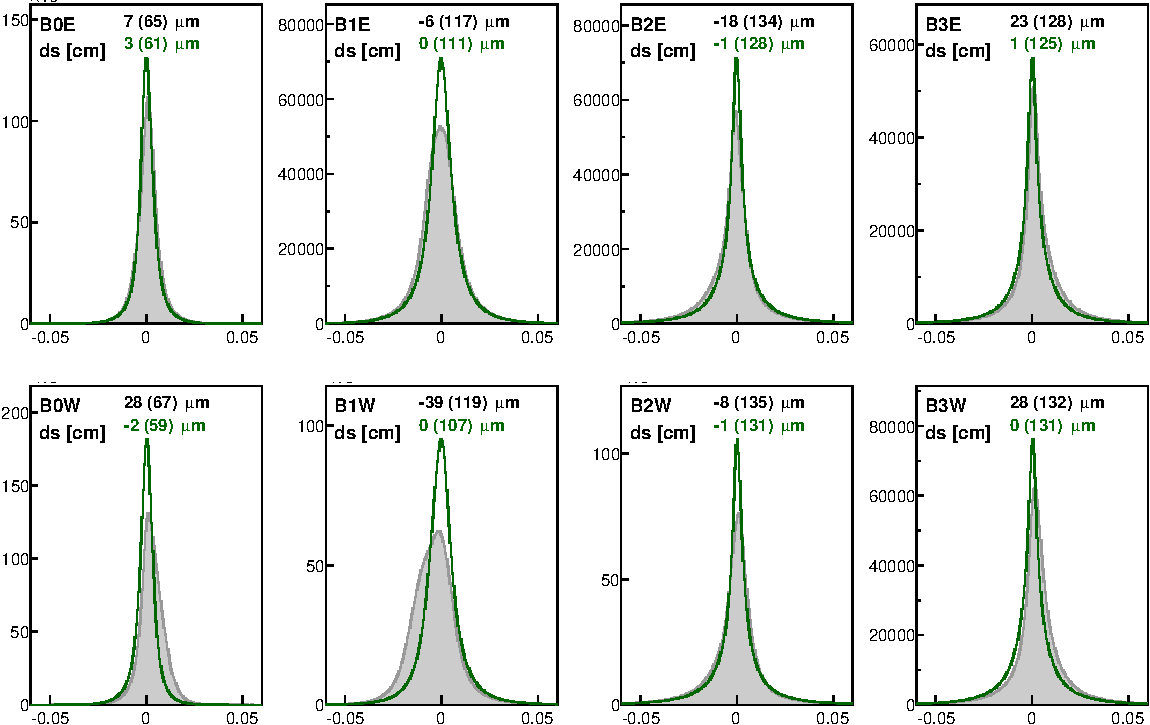
\includegraphics[width=\textwidth]{11vs12/cls0}
  \end{center}
  \caption{$\Delta s$ residuals for half-layer units in the east arm (top) and west arm (bottom) for layers 0-3 (left to right). The gray (green) distributions were filled before (after) halflayer alignment in $x,y$ and $s$. This alignment step led to the geometry labeled 1-2 in table~\ref{tab:history}.}
  \label{fig:hlds}
\end{figure}

\section{Primary vertex, beam center, and DCA}
Fortunately, the GLS technique discussed in section~\ref{sec:trackfit} can also be easily applied to efficiently estimate the primary vertex position. All that is needed is to set up the linear system in a similar way. This is described in section~\ref{sec:vertex}.

\subsection{Fitting the primary vertex} \label{sec:vertex}
In the azimuthal plane, the primary vertex position $(v_x, v_y)$ can be estimated by solving the least-squares system $y_0^{(i)} = -m^{(i)}v_x + v_y$ for $i=1...N$ zero-field tracks, where $y_0 = y(x=0)$ and $m$ is the track slope $\tan(\phi)$. In matrix-vector form, this is $y = X\beta + \epsilon$ where
\begin{equation} \label{eq:vxy}
y = 
 \begin{pmatrix}
 y_0^{(1)}\\
 y_0^{(2)}\\
 \vdots \\
 y_0^{(N)}\\
 \end{pmatrix},
 \qquad
X =
 \begin{pmatrix}
  -m^{(1)}  & 1\\
  -m^{(2)}  & 1\\
  \vdots  & \vdots \\
  -m^{(N)}  & 1
 \end{pmatrix},
 \qquad
\beta = 
 \begin{pmatrix}
 v_x\\
 v_y
 \end{pmatrix}.
\end{equation}
Similarly, for the $z$-vertex we use
\begin{equation} \label{eq:vrz}
y = 
 \begin{pmatrix}
 z_0^{(1)}\\
 z_0^{(2)}\\
 \vdots \\
 z_0^{(N)}\\
 \end{pmatrix},
 \qquad
X =
 \begin{pmatrix}
  -c^{(1)}  & 1\\
  -c^{(2)}  & 1\\
  \vdots  & \vdots \\
  -c^{(N)}  & 1
 \end{pmatrix},
 \qquad
\beta = 
 \begin{pmatrix}
 v_r\\
 v_z
 \end{pmatrix}.
\end{equation}
Since this setup is mathematically identical to that described in section~\ref{sec:lsq}, the primary vertex is found by fitting a set of straight-line tracks in one arm or both arms using equation~\ref{eq:betahat}.

To date, the error on the tracks has not been propagated into the vertex fit. Each track was given an equal (and somewhat arbitrary) error of $\sigma^2 = 0.01$. There is room for improvement here. It is unclear how much difference it would make.

\subsection{Beam center}
\begin{figure}[htb]
  \begin{center}
    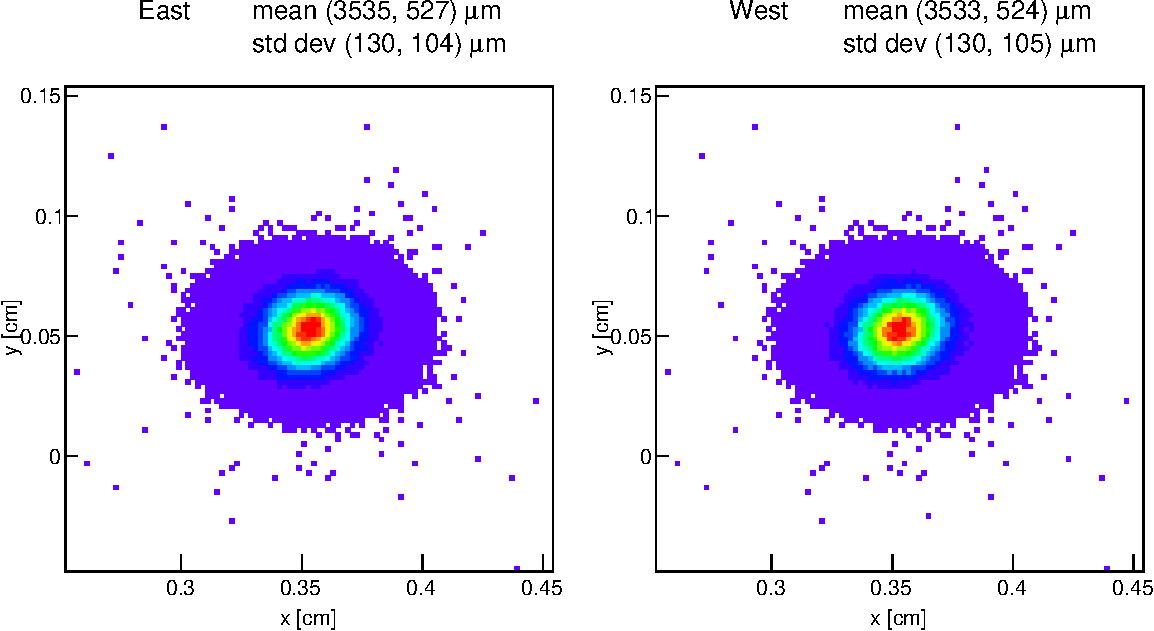
\includegraphics[width=\textwidth]{4/xy_vertex_0}
  \end{center}
  \caption{Primary vertex distribution in the transverse plane from a few hundred thousand peripheral zero-field Run 14 Au$+$Au collisions. Each vertex position was computed as described in section~\ref{sec:vertex}}.
  \label{fig:xyvertex}
\end{figure}

Once the vertex position $(v_x, v_y)$ has been found for many events, it can be histogrammed as shown in figure~\ref{fig:xyvertex}. A measure of central tendency can then be used to estimate the beam center. For this analysis, the median was used in preference to the mean due to its reduced sensitivity to outliers.

For the VTX self-alignment procedure, the beam center was estimated in this way at first iteration, and then fixed for the remainder of the procedure (even though the detector is misaligned). In every single production run, the same beam center position was used. This turned out to be a critical requirement for convergence of the self-alignment procedure, compared to changing the beam center for every production. 

\subsection{Computing the DCA}
Once the primary vertex (or beam center) has been found, each track's distance of closest approach (DCA) can be computed. In the rotated $x$-$y$ coordinates, the impact parameter vector $b'$ is effectively a $\Delta s$ ``residual'' between the track projection and the rotated vertex position $(v_x', v_y')^T = R^{-1} (v_x, v_y)^T$:
\begin{equation} \label{eq:ipxy}
b' = 
\begin{pmatrix}
0 \\
y_0' + m' v_x' - v_y'
\end{pmatrix}
\end{equation}
This can be seen by comparing to equation~\ref{eq:ds}. Using the track unit normal vector $\hat n$
\begin{equation} \label{eq:nhat}
\hat n = 
\begin{pmatrix}
-\sin \phi \\
\cos \phi
\end{pmatrix},
\end{equation}
and the unrotated impact parameter vector $b = R b'$, their inner product defines the $x$-$y$ DCA as a signed scalar quantity: 
\begin{equation} \label{eq:dcaxy}
DCA_{xy} = \hat n \cdot b.
\end{equation}
The $z$ direction is somewhat simpler:
\begin{equation} \label{eq:dcaz}
DCA_{z} = z_0 + c v_x' - v_z.
\end{equation}
Note that this definition of $DCA_{xy}$ does not exactly coincide with the standard PHENIX definition of \texttt{dca2d} (track charge is included in the latter). In zero-field data, $DCA_{xy}$ is broader than the \texttt{dca2d} computed in field-on reconstruction by a factor of three or more. This is because the magnetic field sweeps away very soft particles, reducing effects from scattering and background, and because plotting differentially in $p_T$ in field-on data shows that \texttt{dca2d} becomes narrower by 50\% or more as $p_T$ is increased. 

\begin{figure}[htb]
  \begin{center}
    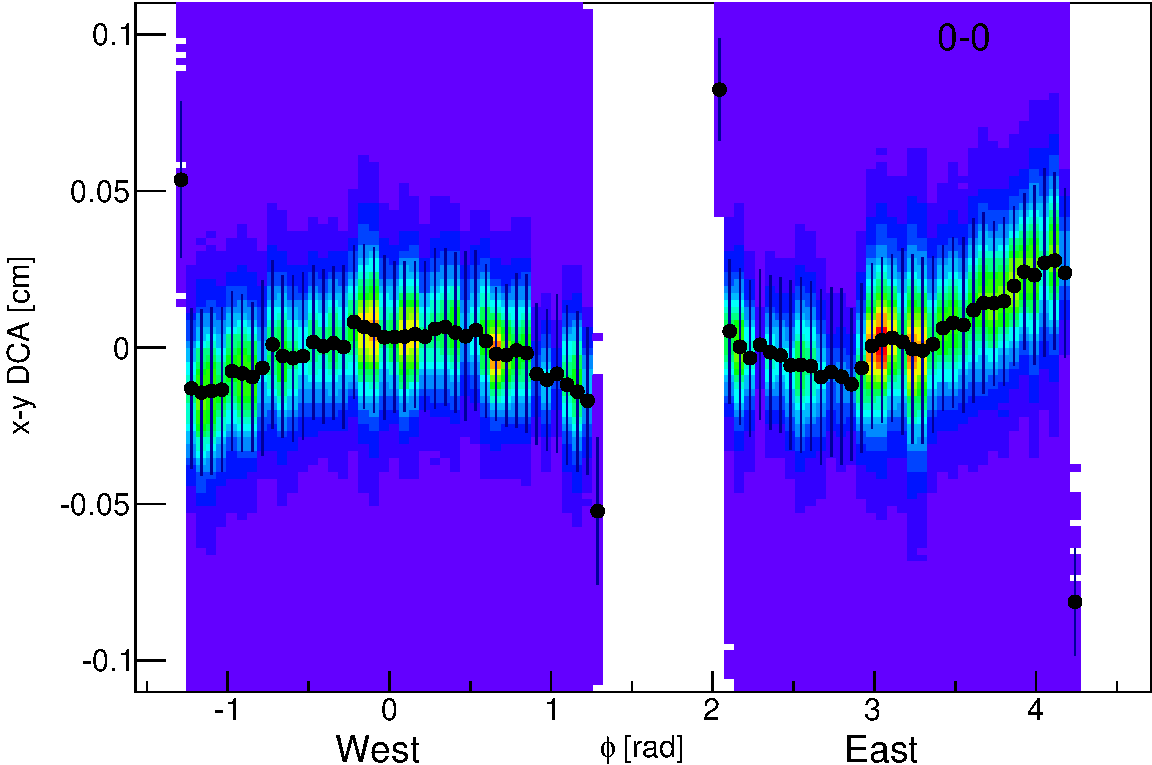
\includegraphics[width=0.48\textwidth]{1/xydca_vs_phi_0}
    \quad
    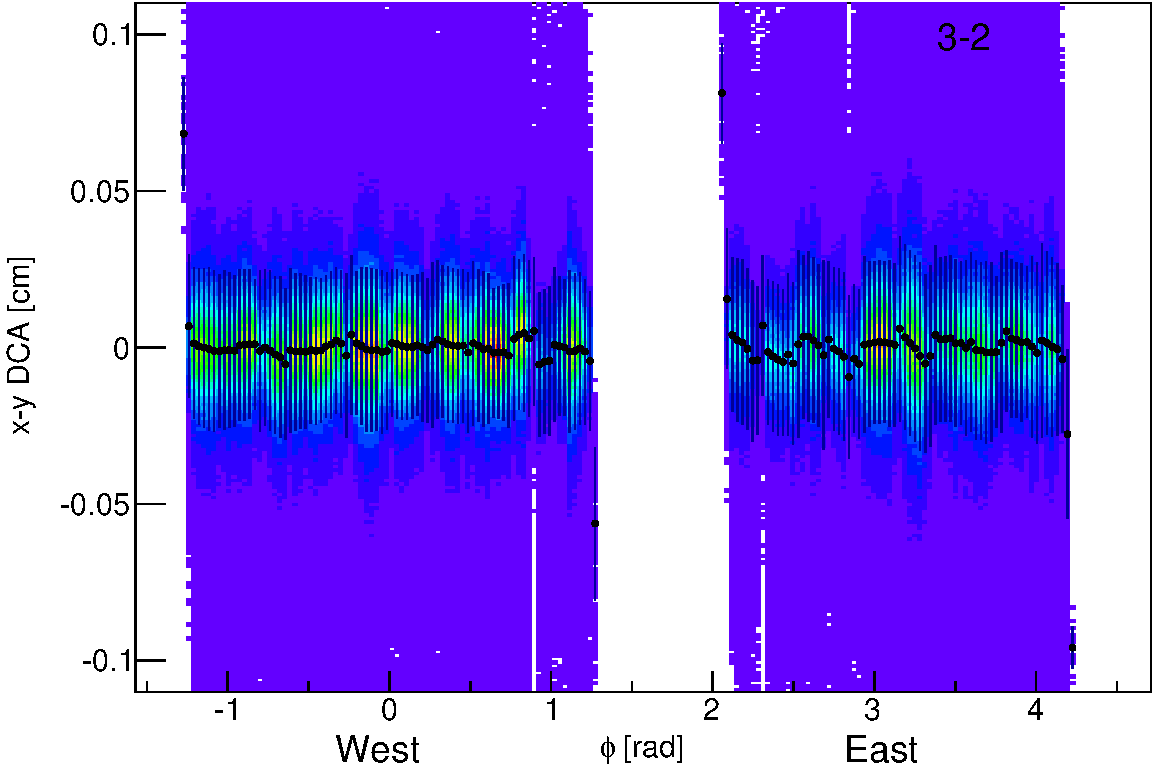
\includegraphics[width=0.48\textwidth]{31vs32/xydca_vs_phi_1}
  \end{center}
  \caption{$DCA_{xy}$ vs. $\phi$ before and after halflayer and ladder alignment.}
  \label{fig:dcavsphi}
\end{figure}
$DCA_{xy}$ vs. $\phi$ is shown in figure~\ref{fig:dcavsphi} before and after halflayer and ladder alignment steps were performed. Before halflayer alignment, a strong cosine pattern is visible, indicating a large-scale misalignment in the $x$ direction. One step of halflayer alignment corrected the majority of the misalignment, allowing progression to ladder-by-ladder alignment.

\section{Mille interface}
The track fit and residual data is given to pede through the Mille class. The VTX interface to \texttt{Mille::mille()} is implemented in \texttt{MilleFunctions.h}. Out of the whole process, this is probably the piece with the steepest learning curve. The manual tends to describe the interface in full pedantic generality, and it can be a bit difficult to specify the discussions there to a concrete application.

\subsection{Local and global fits}
An SvxGeoTrack serves as a ``local fit object'' in Millepede terminology. Two entries are made for each hit (one per residual) by a call to \texttt{Mille::mille()}, and the grouping of entries by track is delimited using \texttt{Mille::end()}.

For each VTX hit, there is a residual in $\Delta s \equiv r\Delta\phi$ and $\Delta z$. Mille takes this residual as an input, along with a set of local and global derivatives. Local derivatives are used by pede to do its own track fits during the optimization procedure. The local derivatives in the transverse plane (corresponding to $\Delta s$) and in the $r$-$z$ plane (corresponding to $\Delta z$) are the derivatives of equations \ref{eq:zrfit} and \ref{eq:yxfit} with respect to their parameters. Since those equations are linear in their parameters (and also their independent variables, for that matter), the derivatives for a track as described in section~\ref{sec:fitdecomp} are simply
\begin{equation} \label{eq:sderlc}
\frac{\partial y'(x')}{\partial y_0'} = 1, \quad 
\frac{\partial y'(x')}{\partial m'} = x' 
\end{equation}
and
\begin{equation} \label{eq:zderlc}
\frac{\partial z(x')}{\partial z_0} = 1, \quad 
\frac{\partial z(x')}{\partial c} = x' 
\end{equation}

Note that there are two separate track fits taking place in the alignment software: the track fits described in section~\ref{sec:trackfit}, and the local fits performed by the pede program during aligmnent. The former provides the residuals needed as input, while the latter is used internally during the optimization to compute changes in the residuals as the detector elements are moved around.

The global derivatives express the degree of change in $\Delta s$ or $\Delta z$ if a detector unit is displaced along a given coordinate. For example, $\partial \Delta s / \partial x = -\sin \phi_{rot}$. 
\begin{table}[htb!]
\centering
\begin{tabular}{c | c | c }
 & $\Delta s$ & $\Delta z$ \\
\hline
$x$ & $-\sin \phi$ & $\cos \phi \cot \theta$ \\
$y$ & $ \cos \phi$ & $\sin \phi \cot \theta$ \\
$z$ & 0 & 1 \\
$s$ & 1 & 0 \\
$r$ & $\Delta s / r$ & $-\cot \theta$ \\
pitch & $-z \cos \phi$ & $-y + z \sin \phi \cot \theta$ \\
yaw & $-z \sin \phi$ & $x - z \cos \phi \cot \theta$ \\
roll & 1 & 0 \\
\hline
\end{tabular}
\caption{Global derivatives of azimuthal and longitudinal residuals with respect to various coordinates.}
\label{tab:dergl}
\end{table}
The global derivatives available in \texttt{MilleFunctions.h} are listed in table \ref{tab:dergl}. The expressions for some global derivatives are self-evident; for others, a fair bit of drawing diagrams, trigonometric manipulation, and some trial and error were involved (especially to get the signs right).

\subsection{Global parameters and labels} \label{sec:labels}
Millepede requires that a unique (but arbitrary) integer label be assigned to a pair consisting of one item from each of the following categories:
\begin{enumerate}
  \item A detector unit (arm, ladder, or halflayer)
  \item An alignment coordinate (any variable in the first column of table \ref{tab:dergl}).
\end{enumerate}
The bidirectional mapping between global parameter labels and these pairs is implemented in \texttt{ParameterDefs.h}, and the label maps can be printed using \texttt{CheckParameters.C}. Not all combinations are useful or supported by the software. In particluar, the pitch, yaw, and roll rotations are currently implemented for arm units only (but there is no reason these rotations could not be implemented for ladders or halflayers in the future.) A list of labels provided to Millepede must represent a linearly independent set; otherwise, Millepede will report a rank deficiency after attempting to solve an underdetermined linear system. 

% For example, trying to align ladders in the set $\{x, y, s, r\}$ will not work because the $\{x, y\}$ and $\{s, r\}$ sets are linear combinations of one another.

\subsection{Constrained optimization}
In the case of the VTX alignment, the number of global parameters ranges from just a handful (for example, three arm rotations $\times$ two arms), to several hundred (for example, ladder-by-ladder alignment in several coordinates). Alignment with a large number of parameters is no problem for Millepede computationally; it has been used successfully to optimize $10^5$ global parameters in just a few hours. 

However, the freedom afforded by a model with many parameters leads to overfitting, which is the tendency for some parameters to take on excessively large values. Overfitting is a general problem arising from attempts to fit a model that is too flexible for the data at hand. Such a model describes the current dataset very well (as measured by $\chi^2$), but generalizes to other similar datasets very poorly. (As an extreme illustration, imagine a 20th-order polynomial fit to a few samples from a smooth distribution.)

The solution is to reduce the effective number of degrees of freedom, either by simplifying the model itself (cutting back free parameters) or by adding external information about the solution. For our case, it is optimal to allow for alignment along all relevant coordinates, so the latter is desirable.

Millepede provides two main ways to constrain the solution. The first is direct regularization using a so-called ``presigma'' parameter, and the second is the ability to fix the sum of an arbitrary list of parameters. Both were used for the Run 14 VTX alignment. 

A presigma of 0.01 was applied to a few ladders with particularly low acceptance/efficiency due to bad electronics. The presigma settings are slightly unintuitive: a smaller value leads to stronger regularization, but a value of zero disables regularization. Any negative value fixes the parameter. So effectively, a very small positive presigma setting has the same effect as a negative value.

Sum constraints are used to fix the average position of a group of detector elements such that their total translation, rotation, or shear is a constant value (usually zero).

Constraint information can be passed to pede in either the steering text file or in one or more dedicated constraint text files. The latter was used for the VTX. The functions to write the constraint file are found in \texttt{ConstraintBuilder.h}. The formatting is simply a \texttt{Parameter} keyword indicating a new block of global parameters, followed by three columns: the parameter label (see section~\ref{sec:labels}), a starting value relative to the current position (always zero in Run 14), and a presigma setting.

For arm alignment, constraints were found to be unnecessary. In \texttt{ConstraintBuilder.h}, there are separate functions to write ladder or halflayer constraints. \texttt{VtxAlign.C} dispatches to one of these functions depending on the \texttt{alignMode} parameter. To modify the existing constraints for a given parameter, there is currently no formal interface; the function bodies were modified directly to change the resulting text files. This was flexible and simple for prototyping and exploration, but there is room for improvement if a more ``proper'' interface is desired.

One downside of applying sum constraints can be illustrated with a problem encountered during the Run 14 alignment. If large corrections are optimal for a subset of the detector units, the remaining units must compensate by absorbing the equal and opposite motion. Moreover, the burden tends to fall very nonuniformly on the more weakly constrained units. For example, during alignment of the ladder radial positions, an entire halflayer (B0E) was brought inwards by several hundred microns. To compensate, a partially-dead edge ladder in B3 was pushed outwards by several mm. That ladder was subsequently recovered to its initial position by hand.

In retrospect, it would have been best to apply the radial constraint differently in this situation: instead of forcing the change of radial ladder positions to sum to zero, the outermost layer, B3, could have been fixed. This would allow the innermost halflayer to make a large radial change without such drastic side-effects in the outer ladders. To correct for distortions, a second alignment pass could be run with sum constraints, once the net radial changes are small enough.



\section{VTX self-alignment workflow: how to do it}
The self-alignment procedure begins with running a zero-field production over a PRDF segment. The output is then filtered in a preprocessing step before alignment. One or more alignment steps are then carried out iteratively. The results from each alignment step are then plotted for analysis.

\subsection{Reconstructing raw data}
There are scripts and production macros located in \texttt{vtx-align/production/\-zerofield} written by Darren McGlinchey to prepare jobs for the condor batch system at RCF. Darren has also prepared a useful README file in the production subdirectories. The reconstruction output is a set of DST files that are then condensed further to TTrees using the Fun4All module located in \texttt{vtx-align/anavtxcluster}. As a final step of the production phase, the TTrees output from \texttt{anavtxcluster} are merged using ROOT's \texttt{hadd} tool.

\subsection{Filtering production output}
The preprocessing of the merged production output trees is carried out by \texttt{FilterData.C}. This fits the tracks and locates a vertex, enabling a loose rejection of outlier events. In addition, a loose cut is placed on residual values so that extreme outliers from bad fits are not fed to Millepede.

\subsection{Running \texttt{VtxAlign.C}}
TODO

\subsection{Orienting the VTX with respect to the central arms}
This part of the alignment is still WIP. When finished, maybe Darren will write a few paragraphs and add a couple plots.

\section{Procedure followed for Run 14}
The general alignment strategy for Run 14 was to begin with larger detector units, then proceed to finer granularity as follows:
\begin{enumerate}
  \item Find the beamcenter in the initial geometry (0-0), and stick with it for the entirety of the process.
  \item align the east and west arms to one another
  \item halflayer alignment
  \item ladder alignment
  \item arm-level rotational self-alignment
\end{enumerate}
A more detailed history of the alignment steps is shown in table \ref{tab:history}. Some of the steps will be described here. The initial beamcenter was found to be (0.353, 0.0528) cm. This is an input to the reconstruction code that remained constant for the entire process. 

\begin{table}[htb!]
\centering
\begin{tabular}{c | c | c | c}
Geom ID & Alias & Description & Constraints \\
\hline
0-0 & hubert-mod & prod 0    & -\\
0-1 & & arm $x,y,z$          & none \\
1-0 & 0-1 & prod 1           & -\\
1-1 & & arm $x,y,z$          & none \\
1-2 & & HL $x,y,z,s$         & $x,y,z,s \in E,W$ sum = 0 \\
2-0 & 1-2 & prod 2           & -\\
2-1 & & HL $x,y,z,s$         & $x,y,z,s \in E,W$ sum = 0 \\
20-2 & & arm $P,Y$           & none \\
21-0 & 20-2 & prod 3         & -\\
21-1 & & L $r,s$             & $^\dagger$ \\
22-0 & 21-1 & prod 4         & -\\
22-11 & & arm $x,y,z,P,Y$    & none \\
\hline
\end{tabular}
\caption{History of alignment steps for Run 14. $^\dagger$For 21-1, all ladder radii were fixed in W arm and in B3E. Radial sums constraints also applied in topmost and bottom-most $\phi$ slices in E arm.}
\label{tab:history}
\end{table}

% \begin{table}[htb!]
% \centering
% \begin{tabular}{c | c | c | c | c | c | c}
% Geom ID & Alias & Description & \multicolumn{2}{c}{$DCA_{xy}$ E [$\mu$m]} 
%                               & \multicolumn{2}{|c}{$DCA_{xy}$ W [$\mu$m]} \\
% (prod-step) & (symlink) &     & $\mu$ & $\sigma$ & $\mu$ & $\sigma$\\
% \hline
% 0-0 & hubert-mod & prod 0    & 63 & 293 & -21 & 261 \\
% 0-1 & & arm $x,y,z$          & 15 & 281 & -12 & 261 \\
% 1-0 & 0-1 & prod 1           & 10 & 280 &  -7 & 257 \\
% 1-1 & & arm $x,y,z$          & 11 & 280 & -10 & 257 \\
% 1-2 & & HL $x,y,z,s$         & -5 & 274 &   4 & 248 \\
% 2-0 & 1-2 & prod 2           & -4 & 273 &   9 & 248 \\
% 2-1 & & HL $x,y,z,s$         & -7 & 273 &   2 & 248 \\
% 2-2 & & L $x,y,z,s$          & -1 & 272 &  -3 & 247 \\
% 3-0 & 2-2-mod & prod 3       & -1 & 274 &  -2 & 247 \\
% 3-1 & & L $x,y,z,s$          & -1 & 274 &   0 & 247 \\
% \colorbox{yellow}{3-2} & & arm $P,Y,R$          &  4 & 272 &  -2 & 244 \\
% \colorbox{yellow}{4-0} & 3-2 & prod 4           &  4 & 270 &  -1 & 241 \\
% 4-1 & & L $s,r$              & -2 & 268 &   0 & 242 \\
% 5-0 & 4-1 & prod             & -2 & 267 &  -1 & 242 \\
% 5-1 & & arm $x,y,z$          &  1 & 266 &  -1 & 242 \\
% \hline
% \end{tabular}
% \caption{History of alignment steps for Run 14.}
% \label{tab:history}
% \end{table}

The goal of the first step is to remove the east-to-west offset (EWO) in $x, y$ and $z$. There is a facility for including these EWOs in the production code, but these were not used (or more precisely, they were set to zero.) The EWO is instead included in the VTX geometry parameter file itself. In order to bring the two arms together, all tracks fits included 

% put 0-0 vs 0-1 geom diff plots here: xy | z.
A large change in the geometry was introduced in this step, particularly in the $z$ coordinate. This can be seen in figure xxx. The zero-field reconstruction was run using the resulting geometry (0-1) in order to reassociate hits to reconstructed standalone tracks. A second identical alignment pass refined the EWO values.


\section{Recommendations}
\begin{itemize}
  \item Use GenerateEvents.C to simulate data with specific misalignments. Then tune VtxAlign.C to correct the misalignment properly. Using the ``sim'' option in VtxAlign.C reduces the sigma parameter passed to Mille so that the $\chi^2/NDF$ is near one.
  \item If pede complains that the $\chi^2$ is too large or too small, its value can be changed by tuning the sigma scaling factor in \texttt{MilleVtx()}.
  \item If pede complains about a rank defect, check that the constraints have not violated any linear independence requirements. 
\end{itemize}
\section{Appendix A: Links to presentations}
TODO
\end{document}
